\documentclass{article}
\usepackage{tikz}
\usetikzlibrary{positioning}

\begin{document}

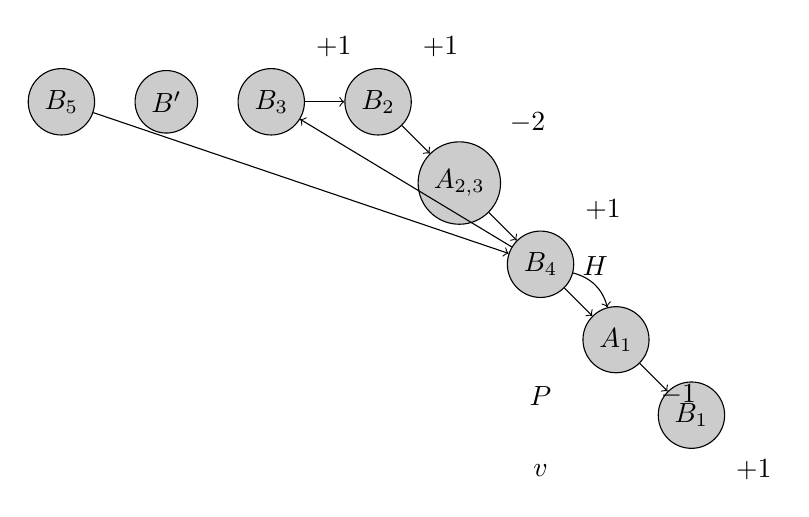
\begin{tikzpicture}[node distance=0.5cm]
    % Define nodes with their labels
    \node[circle,draw,fill=black!20] (B5) {$B_{5}$};
    \node[circle,draw,fill=black!20,right=of B5] (B4) {$B'$};
    \node[circle,draw,fill=black!20,right=of B4] (B3) {$B_{3}$};
    \node[circle,draw,fill=black!20,right=of B3] (B2) {$B_{2}$};
    \node[circle,draw,fill=black!20,below right=of B2] (A23) {$A_{2,3}$};
    \node[circle,draw,fill=black!20,below right=of A23] (B4) {$B_{4}$};
    \node[circle,draw,fill=black!20,below right=of B4] (A1) {$A_{1}$};
    \node[circle,draw,fill=black!20,below right=of A1] (B1) {$B_{1}$};

    % Draw edges between nodes
    \draw[->] (B5) -- (B4);
    \draw[->] (B4) -- (B3);
    \draw[->] (B3) -- (B2);
    \draw[->] (B2) -- (A23);
    \draw[->] (A23) -- (B4);
    \draw[->] (B4) -- (A1);
    \draw[->] (A1) -- (B1);

    % Add labels to the edges
    \node[above right=0.2cm of B2] {$+1$};
    \node[above right=0.2cm of B3] {$+1$};
    \node[above right=0.2cm of A23] {$-2$};
    \node[above right=0.2cm of B4] {$+1$};
    \node[below right=0.2cm of A1] {$-1$};
    \node[below right=0.2cm of B1] {$+1$};

    % Define the path P
    \node[below=1cm of B4] (P) {$P$};
    \draw[->] (B4) to[bend left] node[midway,above] {$H$} (A1);

    % Add labels to the path P
    \node[below=0.5cm of P] {$v$};
\end{tikzpicture}

\end{document}